%%%%%%%%%%%%%%%%%%%%%%%%%%%%%%%%%%%%%%%%%
% Short Sectioned Assignment
% LaTeX Template
% Version 1.0 (5/5/12)
%
% This template has been downloaded from:
% http://www.LaTeXTemplates.com
%
% Original author:
% Frits Wenneker (http://www.howtotex.com)
%
% License:
% CC BY-NC-SA 3.0 (http://creativecommons.org/licenses/by-nc-sa/3.0/)
%
%%%%%%%%%%%%%%%%%%%%%%%%%%%%%%%%%%%%%%%%%

%----------------------------------------------------------------------------------------
%	PACKAGES AND OTHER DOCUMENT CONFIGURATIONS
%----------------------------------------------------------------------------------------

\documentclass[paper=a4, fontsize=11pt]{scrartcl} % A4 paper and 11pt font size

\usepackage[T1]{fontenc} % Use 8-bit encoding that has 256 glyphs
\usepackage{fourier} % Use the Adobe Utopia font for the document - comment this line to return to the LaTeX default
\usepackage[english]{babel} % English language/hyphenation
\usepackage{amsmath,amsfonts,amsthm} % Math packages
\usepackage{amssymb}

\usepackage[T1]{fontenc}
\usepackage[scaled]{beramono}
\usepackage{listings}

\usepackage{algpseudocode}
\usepackage{algorithm}

\usepackage{graphicx}
\DeclareGraphicsExtensions{.png}
\graphicspath{{./imgs/}}

\usepackage{subcaption}

\usepackage{sectsty} % Allows customizing section commands
\allsectionsfont{\normalfont\scshape} % Make all sections centered, the default font and small caps
%\renewcommand{\thesection}{}

% Shove the number into the margin, and places a dot after it.
\makeatletter
\def\@seccntformat#1{\protect\makebox[0pt][r]{\csname
the#1\endcsname.\quad}}
\makeatother

\newtheorem{theorem}{Theorem}[section]
\newtheorem{corollary}{Corollary}[theorem]
\newtheorem{lemma}[theorem]{Lemma}
% For external Lemmas and Theorems
\newtheorem*{theorem*}{Theorem}
\newtheorem*{lemma*}{Lemma}

\usepackage{fancyhdr} % Custom headers and footers
\pagestyle{fancyplain} % Makes all pages in the document conform to the custom headers and footers
\fancyhead{} % No page header - if you want one, create it in the same way as the footers below
\fancyfoot[L]{} % Empty left footer
\fancyfoot[C]{} % Empty center footer
\fancyfoot[R]{\thepage} % Page numbering for right footer
\renewcommand{\headrulewidth}{0pt} % Remove header underlines
\renewcommand{\footrulewidth}{0pt} % Remove footer underlines
\setlength{\headheight}{13.6pt} % Customize the height of the header


\numberwithin{equation}{section} % Number equations within sections (i.e. 1.1, 1.2, 2.1, 2.2 instead of 1, 2, 3, 4)
\numberwithin{figure}{section} % Number figures within sections (i.e. 1.1, 1.2, 2.1, 2.2 instead of 1, 2, 3, 4)
\numberwithin{table}{section} % Number tables within sections (i.e. 1.1, 1.2, 2.1, 2.2 instead of 1, 2, 3, 4)

\setlength\parindent{0pt} % Removes all indentation from paragraphs - comment this line for an assignment with lots of text

\newcommand{\set}[1]{\{#1\}}
\newcommand{\setoneto}[1]{\set{1,2,\ldots,#1}}

\DeclareMathOperator{\OO}{O}
\DeclareMathOperator{\fl}{float}
\DeclareMathOperator{\cut}{\delta}
% \DeclareMathOperator(\ZZ}{\ensuremath{\mathbb{Z}}}
% \DeclareMathOperator(\RR}{\ensuremath{\mathbb{R}}}
%\DeclareMathOperator{\lg}{lg}
\newcommand{\ceil}[1]{\left\lceil#1\right\rceil}
\newcommand{\abs}[1]{\left\lvert#1\right\rvert}
\newcommand{\floor}[1]{\left\lfloor#1\right\rfloor}
\newcommand{\trans}[1]{#1^\intercal}
\newcommand{\opt}[1]{\mathbf{#1}}
%----------------------------------------------------------------------------------------
%	TITLE SECTION
%----------------------------------------------------------------------------------------

\newcommand{\horrule}[1]{\rule{\linewidth}{#1}} % Create horizontal rule command with 1 argument of height

\title{\
    \normalfont\normalsize
    \textsc{University of Waterloo} \\ [25pt] % Your university, school and/or department name(s)
    \horrule{0.5pt} \\[0.4cm] % Thin top horizontal rule
    \huge CS 759 Report:\\
    Killing Time \\
    \horrule{2pt} \\[0.5cm] % Thick bottom horizontal rule
}

\author{Theo Belaire \\ 20415730 \\ Bryan Coutts \\ 20428420} % Your name

\date{\normalsize\today} % Today's date or a custom date

\begin{document}

\maketitle % Print the title


Some terminology, I use the term \textit{included} point to refer to points
that are to be included inside the blob, and \textit{excluded} points to refer
to points that must be on the exterior of the blob.

Unless specified, polygon can mean non-convex polygon. \\

Our algorithm works as follows:
\begin{enumerate}
\item Take the convex hull of the included points.
\item Fix the convex hull, so that no excluded points are in its interior.
\item Compute the radii for each point.
\item Add nearby points to the polygon. 
\item Remove ``crossover'' points.
\item Draw blob around the vertices of the polygon.
\end{enumerate}


\section{Generation of the Convex Hull}
Our code uses the giftwrap algorithm to generate the convex hull.
This runs in $\OO(i^2)$ time, where $i$ is the number of points included in the
set. \\

It works by picking the leftmost point, and calculating the angle that is
formed with each other point in the set, and picking the point that forms
the angle closest to a straight line with the previous point. \\

% TODO nice diagram of in progress giftwrap?
At the conclusion of this step, we have a list of included points in clockwise
order, which forms our polygon.  Currently it's convex.

\section{Point Exclusion}
In this step, we will fix our polygon, so that no excluded point is in its
interior. We will do so by removing triangles from our polytope; this will cause
it to no longer be convex. \\

To test if an excluded point is within our polygon, we use the Jordan Curve
Theorem. One of its consequences is that if we trace a ray from the point in any
direction, it will cross an edge of the polygon an even number of times if and
only if the point is outside the polygon.  This is computationally simple to
check. \\

For each excluded point $p$ in the interior of our polygon, we find the polygon
edge closest to $p$. We consider only the edges whose endpoints $p$ is between.
We then insert $p$ into our list of polygon vertices, between the endpoints of
this edge. This removes the triangle formed by the edge and $p$ from our
polygon.


\section{Calculating Radii}
The \textit{radius} of a point determines how large a circle is used when
drawing the blob around it.  If all the radii were very small, it would not
look very different from just the polygon.  However, we cannot increase the
radii without bound, since we require that the circles for included and
excluded lists cannot intersect.  It looks better if they don't even meet,
so using exactly half the distance to the nearest point of the opposite type
is not quite the best.
Instead, we have a tunable parameter,
which is around 2.5. %TODO

Also, we don't want to create a scenario where we close the ``neck''
on an exterior point that was inside the convex hull, trapping it inside.

\begin{figure}[h]
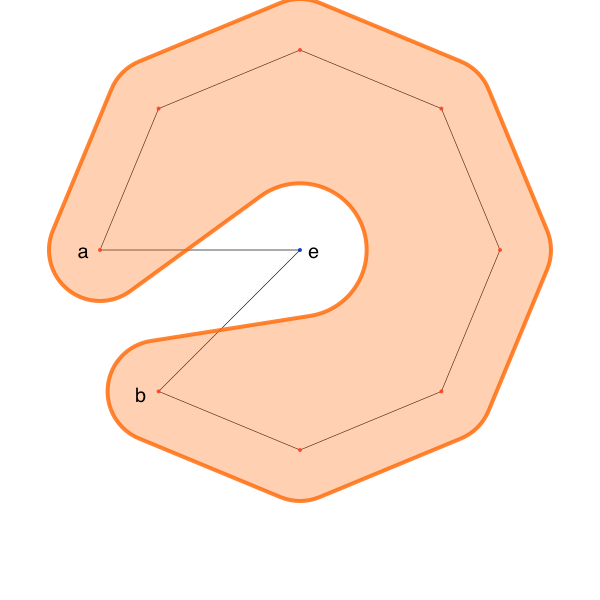
\includegraphics[width=0.5\textwidth]{torus_bitten}
\centering
\caption{``An example of why we need the second rule''}
\label{fig:neck}
\end{figure}

See~\ref{fig:neck} for an example.

The only time we need to restrict radii of interior points based on other
interior points are when the straight line between the two is not
contained within the polygon.  Same goes for exterior points that have a line
that is not fully outside of the polygon.

The way we check this is to see if the line between the two points intersects
any of the lines that make up the polygon.



\section{Absorbing points near lines}
Once we have all the radii, we almost know the final shape of the blob.

We need to check if there are any exterior points where the circle
formed with their radii intersects with the blob.
So that we can properly avoid them, we will add the excluded points to
the boundary list.

\begin{figure}
        \centering
        \begin{subfigure}[b]{0.5\textwidth}
                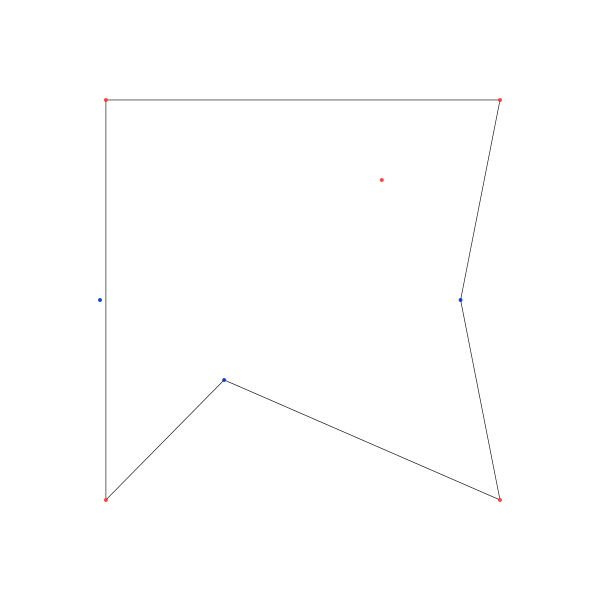
\includegraphics[width=\textwidth]{before_caving}
                \caption{Before}
                \label{fig:before}
        \end{subfigure}%
        ~ %add desired spacing between images, e. g. ~, \quad, \qquad, \hfill etc.
          %(or a blank line to force the subfigure onto a new line)
        \begin{subfigure}[b]{0.5\textwidth}
                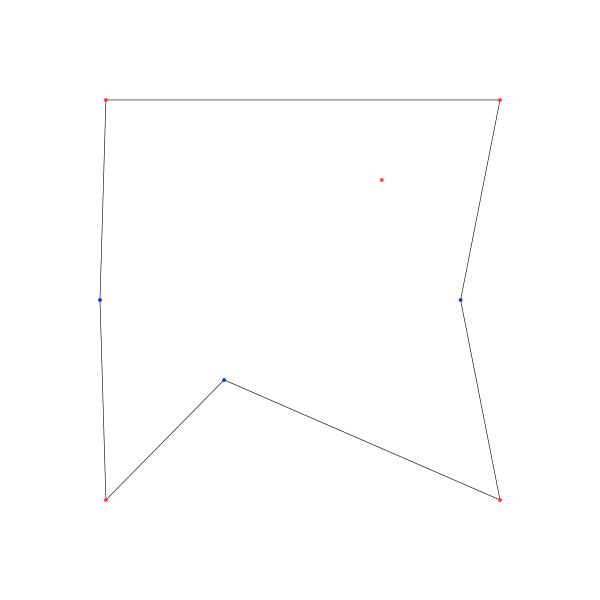
\includegraphics[width=\textwidth]{after_caving}
                \caption{After}
                \label{fig:after}
        \end{subfigure}
        \caption{Before and After caving}\label{fig:caving}
\end{figure}


\section{Uncrossing}

\section{Arc computation}
Once we have a final boundary, and radii, we can draw the blob.

For each edge $uv$, we consider a pair of circles centered at
$u$ and $v$, with the radii $r_u$ and $r_v$.

Consider as if we were to take a piece of string and wrap it around
the outside of these circles.
It would have three segments,
first when it was in contact with the first circle,
then it would leave and travel along a line tangent to both circles,
then it would arrive at the second circle
and travel along it before leaving somewhere on the other side.




% \begin{figure}[h]
% \includegraphics[width=\textwidth]{7/folder}
% \caption{''It's number 7''}
% \end{figure}
\end{document}
